\subsection{OpenML 基准上的操控实验}
\label{sec:semi_synthetic_results}

上下文扰动轨道包含 72 个 OpenML-CC18 分类数据集和 35 个 OpenML-CTR23 回归数据集；分布偏移轨道分别包含 35 个和 33 个数据集。干净数据性能使用原始上下文与输入计算。

% Original sources for every named Table 1 and Table 4 predictor. The
% non-printing citations preserve the compact result layout while ensuring
% that each baseline has a corresponding bibliography entry.
\nocite{cox1958binary,hoerl1970ridge,cortes1995svm,drucker1996svr,
cover1967knn,breiman2001randomforests,ke2017lightgbm,
prokhorenkova2018catboost,chen2016xgboost,rumelhart1986backprop,
gorishniy2021fttransformer,gorishniy2025tabm,thielmann2024tabularnn,
ahamed2024mambatab,holzmueller2024realmlp,qu2026tabiclv2,
grinsztajn2026tabpfn3technicalreport,wang2026limix2m,ma2025tabdpt}

表~\ref{tab:overall-performance} 比较了 13 个常规或神经网络基线与四个冻结的表格基础模型：LimiX-2M、TabICL-v2、TabPFN-v3 和 TabDPT v1.2。相对于 Base，Shared 改善了所有非零强度下的扰动与偏移指标；Specific 在每项比较中进一步提升性能。干净数据得分基本不变。基线配置、引用以及覆盖完整测试套件的 LimiX 兼容性方案见附录~\ref{app:baseline_details}。

\paragraph{OpenML 任务上的强度响应。}
图~\ref{fig:semisynthetic-strength} 报告全部五个强度，并对数据集以及五种扰动或七种偏移类别赋予相同权重。强度为零时，三种配置的性能接近。随着强度增加，Base 下降最快，Shared 持续减缓下降，Specific 则进一步改善；在每个非零强度下，Specific 在全部八个面板中均取得最高得分。

\subsection{全合成稳健性实验}
\label{sec:results}

\paragraph{实验方案与基线。}
我们在 12 个合成问题类别上评估固定五槽位的 Shared 接口。这些问题由五种具有相关特征与受控目标的数据生成过程产生。每个问题类别均在五个强度和三个随机种子下测试。比较对象包括附录~\ref{app:baseline_details} 所列的九种稳健学习、对抗训练与分布适配基线。对齐的评估单元在分类任务中使用 AUROC，在回归任务中使用 $R^2$。

\ifdefined\ICLRLayout
\begin{figure}[H]
  \centering
  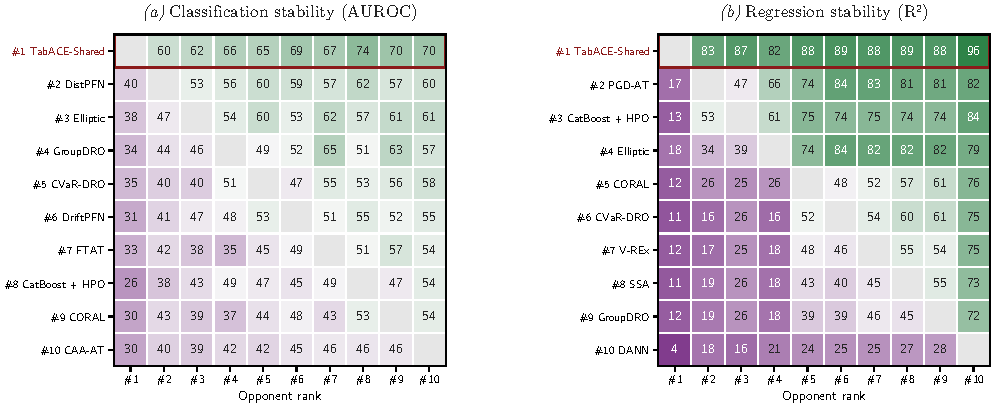
\includegraphics[width=0.88\textwidth]{figures/tabace_synthetic_stability.pdf}
  \caption{在 180 个对齐的“随机种子--DGP--场景”实验单元上的成对稳定性。分类使用经机会水平校正的 AUROC 边际退化，回归使用归一化 $R^2$ 退化。单元格表示行方法取得较小性能下降的频率；差异不超过 $0.001$ 时记为平局。}
  \label{fig:synthetic-stability}
\end{figure}

\begin{figure}[H]
  \centering
  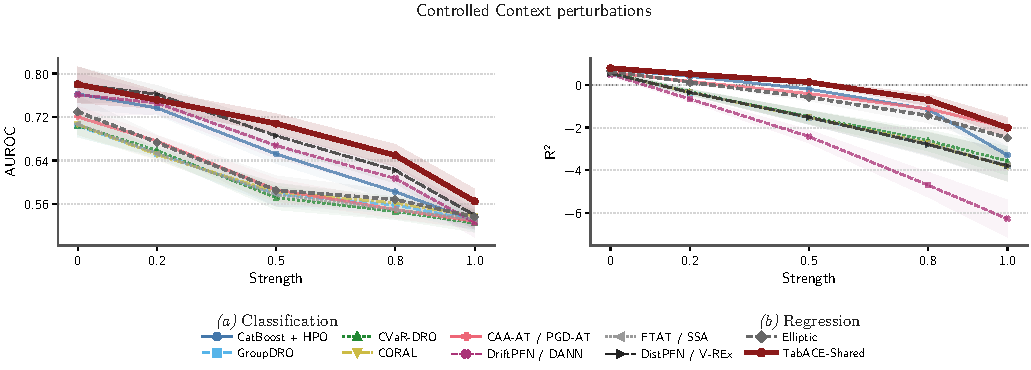
\includegraphics[width=0.94\textwidth]{figures/tabace_controlled_response.pdf}
  \caption{全合成设置下对受控上下文扰动的响应。各面板分别报告分类 AUROC 与回归 $R^2$；曲线汇总五种扰动类别上的对齐实验单元，阴影带表示 $95\%$ bootstrap 区间。}
  \label{fig:synthetic-controlled-response}
\end{figure}
\fi

\paragraph{稳定性。}
对于每个“随机种子--DGP--场景”实验单元，我们对四个非零强度取平均，并分别以干净数据 AUROC 的判别裕量和干净数据 $R^2$ 对分类与回归的性能退化进行归一化。具体定义见附录~\ref{app:metrics_reporting}。图~\ref{fig:synthetic-stability} 报告 180 个对齐实验单元上的成对胜率。TabACE-Shared 在分类和回归中均排名第一，平均胜率分别为 $67.0\%$ 和 $87.6\%$。

\ifdefined\ICLRLayout
\paragraph{强度响应。}
图~\ref{fig:synthetic-controlled-response} 报告受控上下文扰动下的分类 AUROC 与回归 $R^2$。曲线对对齐的 DGP、问题与随机种子单元赋予相同权重，并给出 $95\%$ bootstrap 区间。从强度 $0.5$ 起，TabACE-Shared 取得最高的分类 AUROC。上下文数量与聚合规则的消融实验见附录。

\subsection{补充实验}
\label{sec:additional-experiments}

\paragraph{自然分布偏移。}
Folktables~\citep{ding2021folktables} 提供了 2018 年从加利福尼亚州到密歇根州的地理偏移，以及加利福尼亚州内从 2014 年到 2018 年的时间偏移。表~\ref{tab:natural-shifts} 报告 Employment、Income 和 TravelTime 任务上的 ID 与 OOD Accuracy。Specific 在所有设置下均取得最高得分。

\definecolor{sharedblue}{RGB}{31,84,147}
\definecolor{specificred}{RGB}{213,94,0}

\begin{table}[H]
  \centering
  \begin{minipage}[t]{0.61\textwidth}
    \vspace{0pt}
    \centering
    \caption{自然地理偏移与时间偏移下的 ID 和 OOD Accuracy。}
    \label{tab:natural-shifts}
    \small
    \setlength{\tabcolsep}{4.0pt}
    \renewcommand{\arraystretch}{1.02}
    \begin{tabular}{@{}llccc@{}}
      \toprule
      方法 & 域 & Employment & Income & TravelTime \\
      \midrule
      \multicolumn{5}{@{}l}{\textit{地理：California $\rightarrow$ Michigan（2018）}} \\
      Base & ID  & 0.7922 & 0.7888 & 0.5912 \\
           & OOD & 0.8043 & 0.7655 & 0.5472 \\
      Shared & ID
        & \textcolor{sharedblue}{0.7948} & \textcolor{sharedblue}{0.7951}
        & \textcolor{sharedblue}{0.5945} \\
           & OOD
        & \textcolor{sharedblue}{0.8078} & \textcolor{sharedblue}{0.7832}
        & \textcolor{sharedblue}{0.5961} \\
      Specific & ID
        & \textcolor{specificred}{\textbf{0.7979}}
        & \textcolor{specificred}{\textbf{0.7955}}
        & \textcolor{specificred}{\textbf{0.6002}} \\
           & OOD
        & \textcolor{specificred}{\textbf{0.8089}}
        & \textcolor{specificred}{\textbf{0.7840}}
        & \textcolor{specificred}{\textbf{0.6034}} \\
      \addlinespace[2pt]
      \multicolumn{5}{@{}l}{\textit{时间：California 2014 $\rightarrow$ 2018}} \\
      Base & ID  & 0.7704 & 0.7926 & 0.5951 \\
           & OOD & 0.7847 & 0.7844 & 0.5908 \\
      Shared & ID
        & \textcolor{sharedblue}{0.7751} & \textcolor{sharedblue}{0.7968}
        & \textcolor{sharedblue}{0.6032} \\
           & OOD
        & \textcolor{sharedblue}{0.7900} & \textcolor{sharedblue}{0.7937}
        & \textcolor{sharedblue}{0.5975} \\
      Specific & ID
        & \textcolor{specificred}{\textbf{0.7757}}
        & \textcolor{specificred}{\textbf{0.7980}}
        & \textcolor{specificred}{\textbf{0.6061}} \\
           & OOD
        & \textcolor{specificred}{\textbf{0.7916}}
        & \textcolor{specificred}{\textbf{0.7947}}
        & \textcolor{specificred}{\textbf{0.5981}} \\
      \bottomrule
    \end{tabular}
  \end{minipage}\hfill
  \begin{minipage}[t]{0.36\textwidth}
    \vspace{0pt}
    \centering
    \caption{上下文集成相对于各未经修改的常规预测器的增益。}
    \label{tab:traditional-backbone-gains}
    \small
    \setlength{\tabcolsep}{4.0pt}
    \renewcommand{\arraystretch}{1.02}
    \begin{tabular}{@{}lcc@{}}
      \toprule
      \multicolumn{3}{c}{分类：$\Delta$Accuracy $\uparrow$} \\
      \cmidrule(lr){1-3}
      预测器 & Shared & Specific \\
      \midrule
      kNN & \textcolor{sharedblue}{+0.0167}
        & \textcolor{specificred}{\textbf{+0.0227}} \\
      Logistic & \textcolor{sharedblue}{+0.0069}
        & \textcolor{specificred}{\textbf{+0.0287}} \\
      CatBoost & \textcolor{sharedblue}{+0.0145}
        & \textcolor{specificred}{\textbf{+0.0287}} \\
      MLP & \textcolor{sharedblue}{+0.0107}
        & \textcolor{specificred}{\textbf{+0.0285}} \\
      \addlinespace[5pt]
      \multicolumn{3}{c}{回归：$\Delta R^2$ $\uparrow$} \\
      \cmidrule(lr){1-3}
      预测器 & Shared & Specific \\
      \midrule
      kNN & \textcolor{sharedblue}{+0.0203}
        & \textcolor{specificred}{\textbf{+0.0654}} \\
      Ridge & \textcolor{sharedblue}{+0.1425}
        & \textcolor{specificred}{\textbf{+0.1966}} \\
      CatBoost & \textcolor{sharedblue}{+0.1279}
        & \textcolor{specificred}{\textbf{+0.1740}} \\
      MLP & \textcolor{sharedblue}{+0.0499}
        & \textcolor{specificred}{\textbf{+0.1645}} \\
      \bottomrule
    \end{tabular}
  \end{minipage}
\end{table}


\begin{figure}[H]
  \centering
  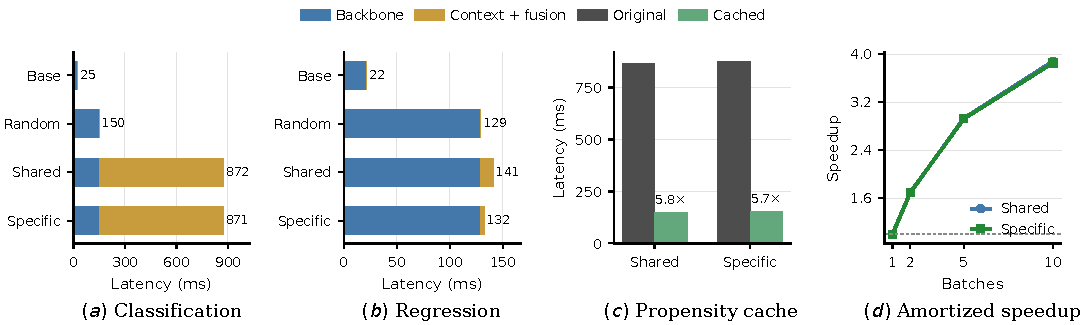
\includegraphics[width=0.96\textwidth]{figures/tabace_inference_cost_ablation.pdf}
  \caption{五个替代上下文和单独评估的 Base 分支的推理成本消融。面板 (a--b) 分解中位延迟；(c) 比较原始推理与缓存推理；(d) 在摊销加速比中计入一次性缓存建立成本。}
  \label{fig:inference-cost}
\end{figure}
\else
\paragraph{强度响应。}
图~\ref{fig:synthetic-controlled-response} 报告受控上下文扰动下的分类 AUROC 与回归 $R^2$。曲线对对齐的 DGP、问题与随机种子单元赋予相同权重，并给出 $95\%$ bootstrap 区间。从强度 $0.5$ 起，TabACE-Shared 取得最高的分类 AUROC。上下文数量与聚合规则的消融实验见附录。
\fi

\ifdefined\ICLRLayout\else
\subsection{补充实验}
\label{sec:additional-experiments}

\paragraph{自然分布偏移。}
Folktables~\citep{ding2021folktables} 提供了 2018 年从加利福尼亚州到密歇根州的地理偏移，以及加利福尼亚州内从 2014 年到 2018 年的时间偏移。表~\ref{tab:natural-shifts} 报告 Employment、Income 和 TravelTime 任务上的 ID 与 OOD Accuracy。Specific 在所有设置下均取得最高得分。
\fi

\paragraph{常规预测器兼容性。}
将同一上下文集成接口应用于 kNN、Logistic/Ridge、CatBoost 和 MLP 后，Shared 在所有预测器上均提高了分类 Accuracy 和回归 $R^2$；Specific 则在全部八项比较中进一步提升性能（表~\ref{tab:traditional-backbone-gains}）。

\paragraph{推理成本。}
对于固定五上下文 Shared 库，图~\ref{fig:inference-cost} 将实际运行延迟分解为六次主干模型前向过程（Base 加五个替代上下文）以及上下文构造/融合。缓存可复用的倾向量使重复推理速度提高约 $5.7\times$。计入一次性缓存构造成本后，在十个批次上的摊销加速比仍约为 $3.9\times$。

\FloatBarrier
